%%%%%%%%%%%%%%%%%%%%%%%%%%%%%%%%%%%%%%%%%%%%%%%%%%%%%%%%%%%
%
%--------------CAPÍTULO 5 - RESULTADOS E DISCUSSÃO----------
%
%
\chapter{Resultados e Discussão}
\label{cap:resultados}

Este capítulo apresenta os resultados na ordem em que as etapas foram executadas (Capítulo~\ref{cap:materiais-metodos}). A Seção~\ref{sec:res-poc} mostra o resultado da prova de conceito com o detector pré-treinado. A Seção~\ref{sec:res-roteamento} apresenta o treinamento da rede de roteamento e a análise de seus mapas de oclusão. As Seções~\ref{sec:res-especialistas} e~\ref{sec:res-baseline} trazem as métricas de validação cruzada dos especialistas e do baseline monolítico, e a Seção~\ref{sec:res-comparacao-metricas} compara as duas abordagens com base nessas métricas. A Seção~\ref{sec:res-videos} apresenta a avaliação nos vídeos de teste independentes, e a Seção~\ref{sec:res-discussao} discute o conjunto dos resultados e suas limitações.

\section{Prova de Conceito com Detector Pré-Treinado}
\label{sec:res-poc}

A Figura~\ref{fig:poc-sheep} mostra o resultado típico do YOLOv8m pré-treinado no COCO aplicado a um quadro da câmera frontal durante o dia, com as detecções filtradas pela classe \textit{sheep}. Dos oito animais da baia principal, o modelo detectou apenas dois, com confianças de 0,27 e 0,48. Os testes com imagens noturnas e com a perspectiva superior também tiveram desempenho insatisfatório, sem que o modelo detectasse o rebanho completo.

\begin{figure}[htb]
\centering
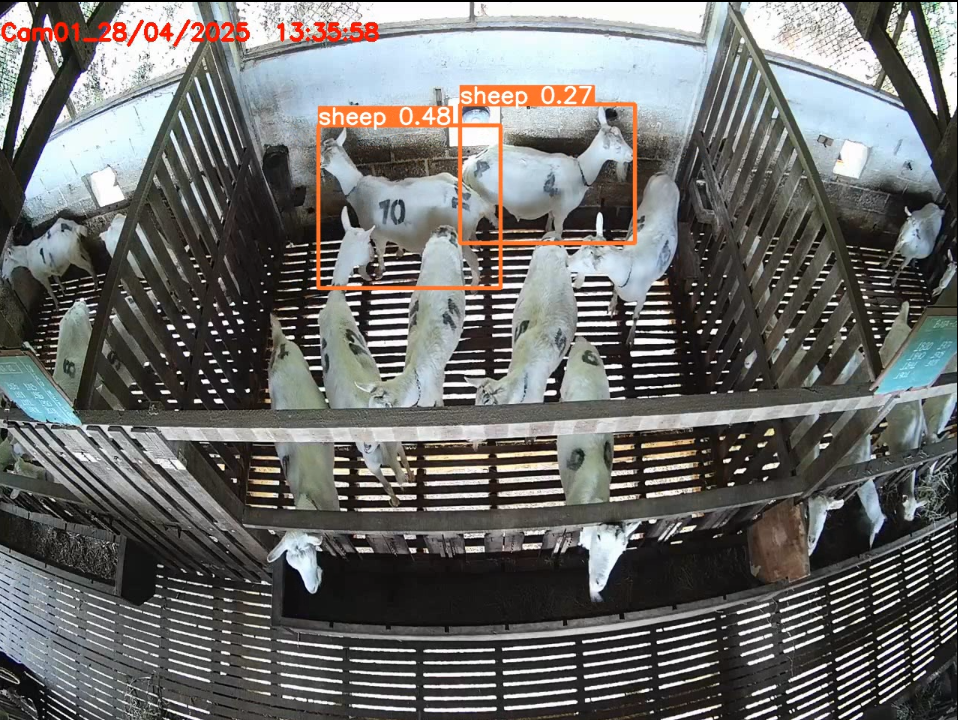
\includegraphics[width=0.75\textwidth]{figs/sheep-test.png}
\caption{Prova de conceito: YOLOv8m pré-treinado no COCO, sem ajuste, com detecções filtradas pela classe \textit{sheep}. Apenas dois dos oito animais da baia principal foram detectados.}
\label{fig:poc-sheep}

Fonte: Elaborada pelo autor.
\end{figure}

Esse desempenho era esperado. O COCO não tem caprinos, e cabras \textit{Saanen} vistas de cima ou em diagonal, através das grades de uma baia, têm aparência diferente da dos ovinos que o modelo aprendeu a reconhecer. À noite, a diferença aumenta, porque as imagens em infravermelho são monocromáticas, ao passo que o COCO é formado por fotografias coloridas. O teste confirmou que seria necessário construir uma base própria e treinar detectores para o domínio. Como teve caráter apenas exploratório, esse teste não é usado como base de comparação no restante do capítulo; esse papel cabe ao baseline monolítico (Seção~\ref{sec:res-baseline}).

\section{Rede de Roteamento}
\label{sec:res-roteamento}

\subsection{Treinamento e Desempenho de Validação}
\label{subsec:res-treino-roteamento}

O treinamento da EfficientNet-B0 foi interrompido pela parada antecipada na nona época. A Figura~\ref{fig:curva-roteamento} mostra a perda de treino e de validação ao longo das épocas. A perda de validação ficou próxima de zero já a partir da segunda época e não voltou a cair o suficiente para reiniciar a contagem da paciência, o que levou à parada sete épocas depois. A perda de treino oscilou mais, com picos na quarta e na sexta épocas, efeito esperado do aumento de dados aplicado só ao treino, e também se aproximou de zero nas últimas épocas.

\begin{figure}[htb]
\centering
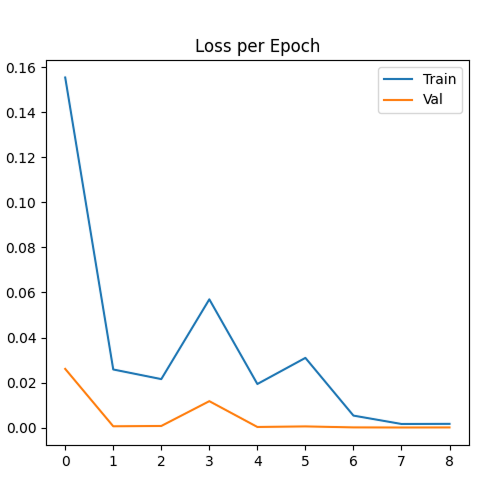
\includegraphics[width=0.5\textwidth]{figs/learning_curves.png}
\caption{Perda de treino (\textit{Train}) e de validação (\textit{Val}) da rede de roteamento por época. A numeração das épocas no eixo horizontal começa em zero.}
\label{fig:curva-roteamento}

Fonte: Elaborada pelo autor.
\end{figure}

No conjunto de validação, com 272 imagens, a rede classificou corretamente todas as imagens dos quatro cenários: precisão, revocação e F1-\textit{score} foram iguais a 1,00 em todas as classes. A convergência rápida e o acerto total indicam que distinguir os quatro cenários é uma tarefa fácil para a rede. Isso faz sentido, já que a diferença entre perspectiva frontal e superior muda a geometria inteira da cena, e a diferença entre dia e noite muda a cor da imagem inteira.

Esse resultado precisa ser lido com cautela por dois motivos já apontados na Seção~\ref{subsec:base-roteamento}. O primeiro é que a divisão entre treino e validação dessa base foi aleatória por quadro, de modo que quadros próximos de um mesmo vídeo podem estar nos dois conjuntos. O segundo é que a base é desbalanceada, e a classe Frontal Noite tem apenas 16 imagens de validação. O acerto total, portanto, não prova que a rede generalize para vídeos novos. Essa verificação é feita na Seção~\ref{subsec:res-roteamento-videos}, com os vídeos de teste independentes.

\subsection{Mapas de Sensibilidade por Oclusão}
\label{subsec:res-oclusao}

A Figura~\ref{fig:oclusao} mostra os mapas de sensibilidade por oclusão de uma imagem de cada cenário, sobrepostos às imagens. As cores quentes (amarelo e vermelho) indicam as regiões cuja oclusão mais altera a saída da rede para a classe prevista, e as cores frias (azul), as regiões que pouco influenciam a decisão. A rede previu corretamente o cenário das quatro imagens.

\begin{figure}[htb]
\centering
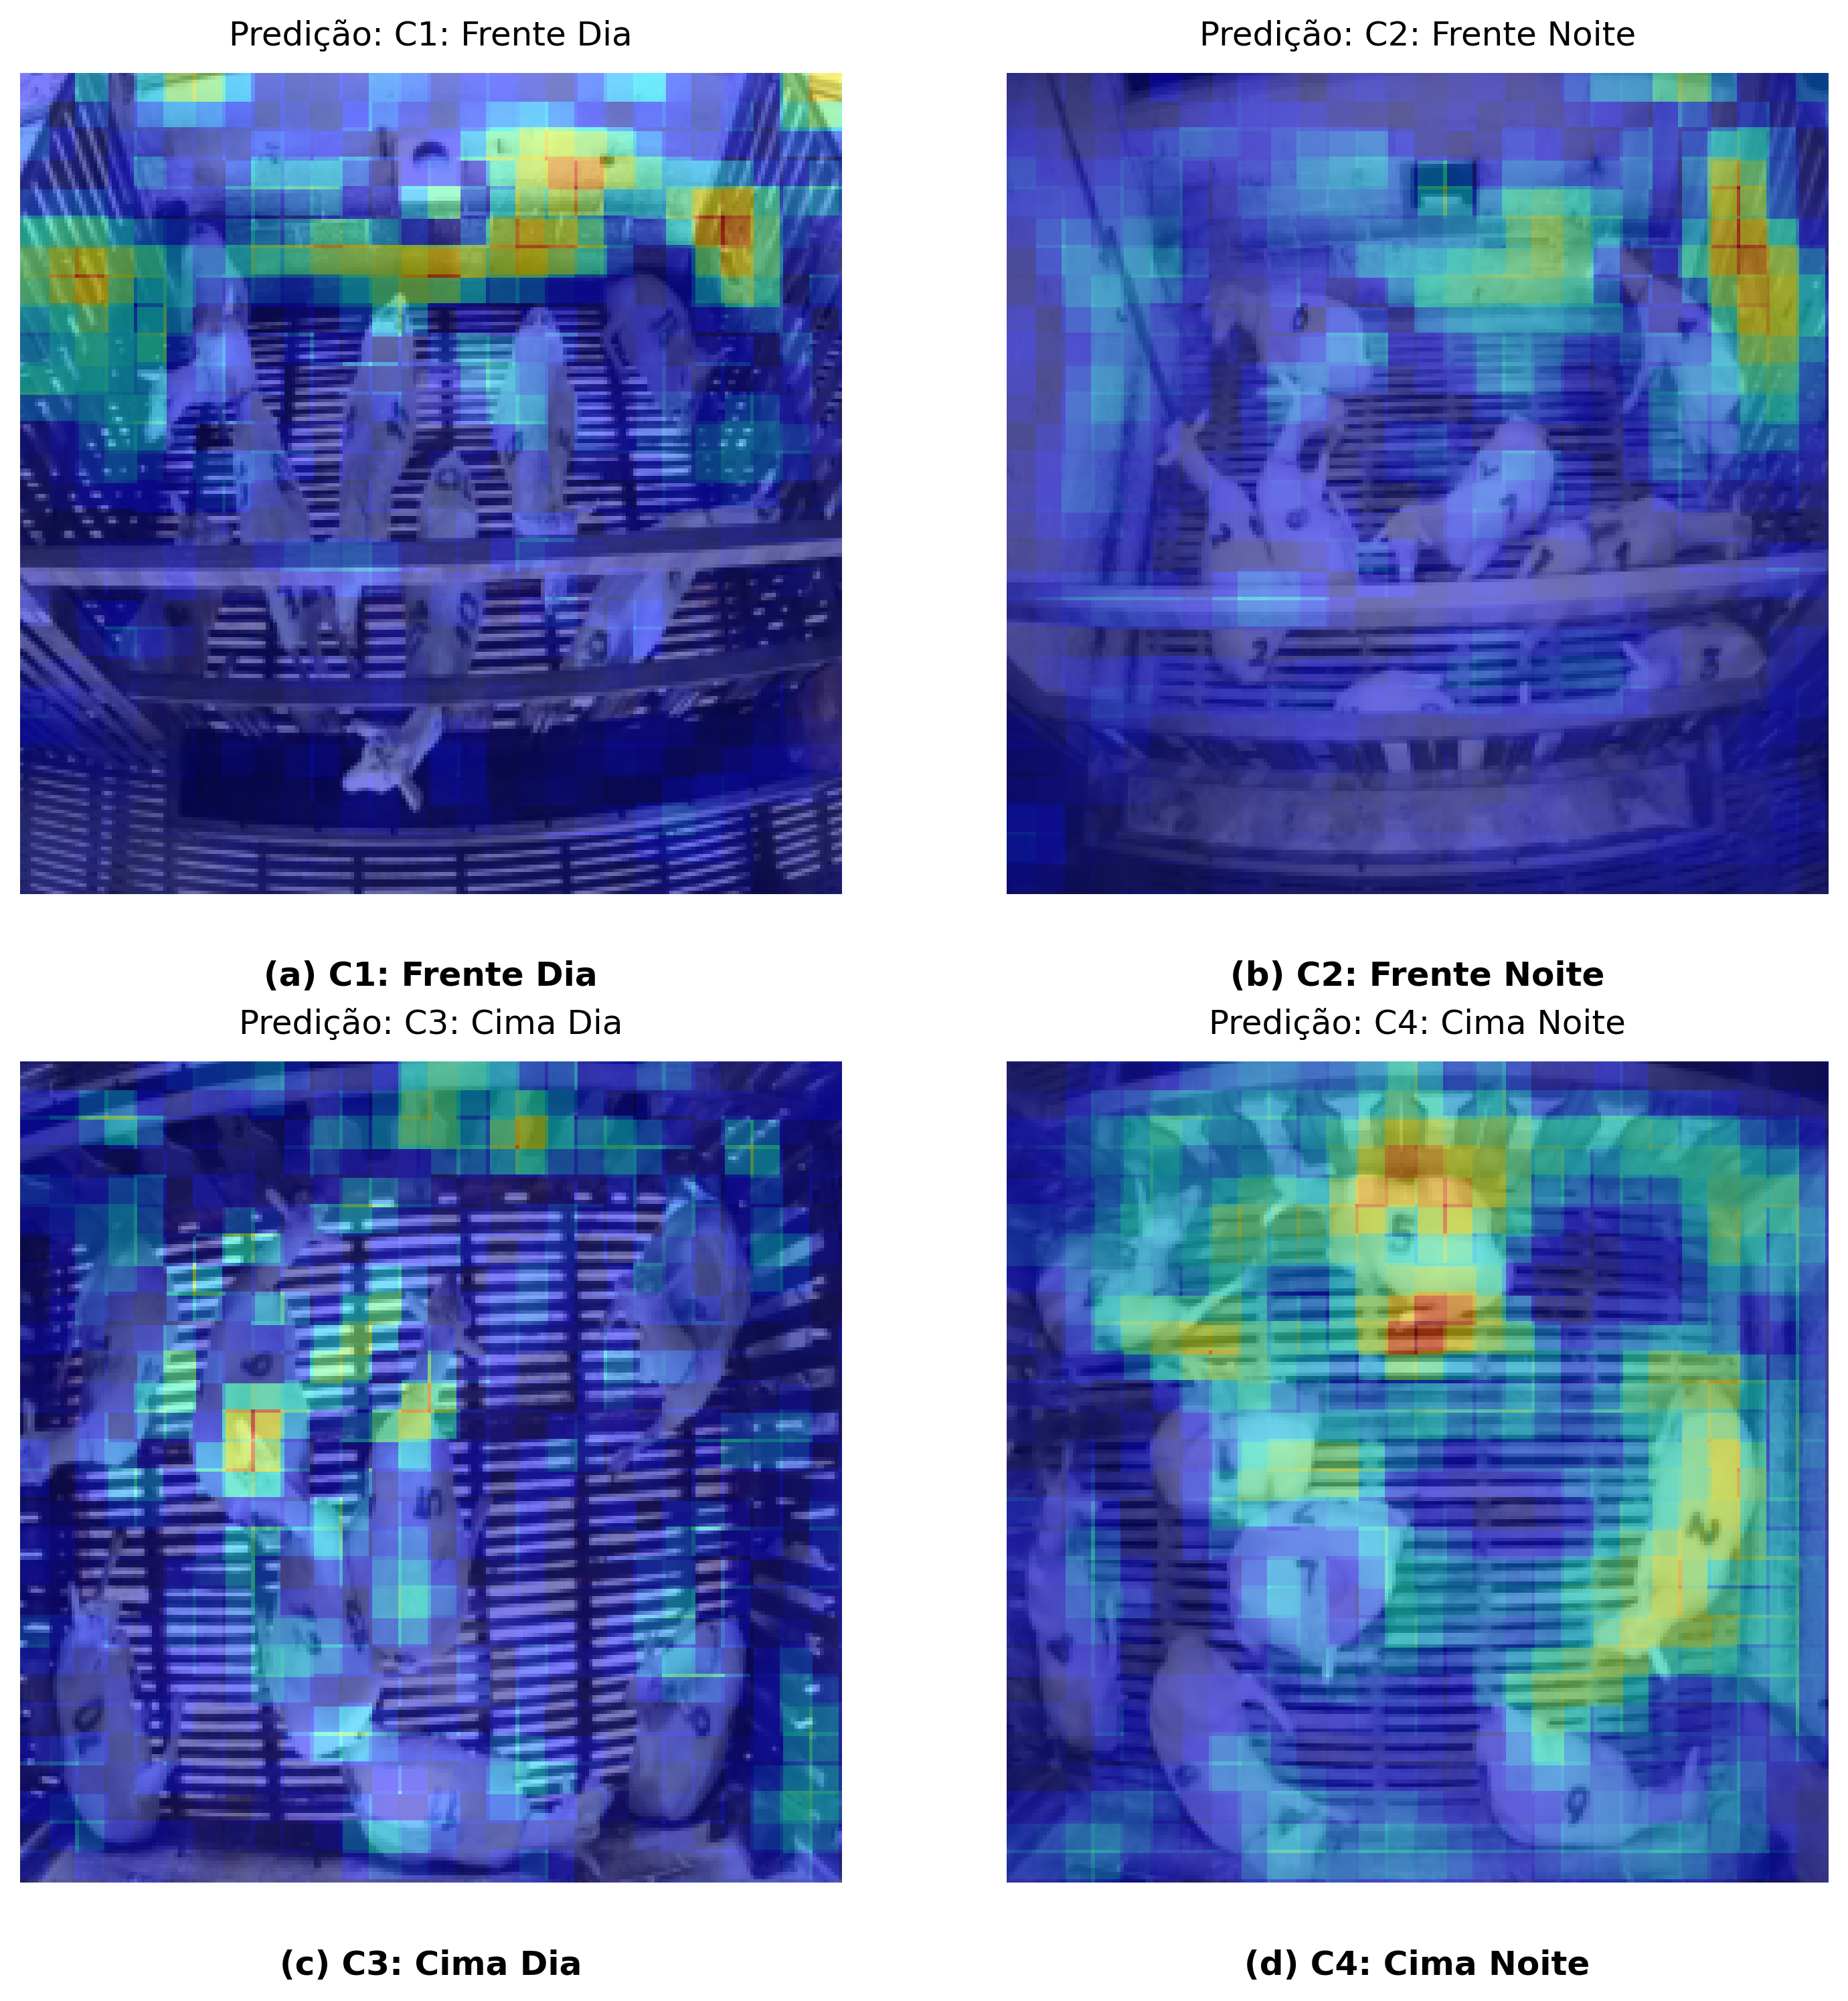
\includegraphics[width=0.85\textwidth]{figs/occlusion_2x2_blended.png}
\caption{Mapas de sensibilidade por oclusão da rede de roteamento, sobrepostos às imagens de entrada: (a) Frontal Dia; (b) Frontal Noite; (c) Superior Dia; (d) Superior Noite. Cores quentes indicam maior influência na decisão.}
\label{fig:oclusao}

Fonte: Elaborada pelo autor.
\end{figure}

Nos dois cenários frontais, a rede se apoiou sobretudo na estrutura da baia. Em Frontal Dia (Figura~\ref{fig:oclusao}a), as regiões mais relevantes ficam na faixa superior da imagem, sobre a parede do fundo e a parte alta das grades laterais, e quase não há relevância sobre os corpos dos animais ou sobre o cocho na parte inferior. Em Frontal Noite (Figura~\ref{fig:oclusao}b), o padrão é parecido: a região mais relevante é a grade do lado direito e a parte superior da parede, enquanto os animais aparecem em azul.

Nos cenários superiores, o padrão é menos uniforme. Em Superior Dia (Figura~\ref{fig:oclusao}c), o mapa é difuso: há pontos de relevância moderada espalhados sobre o piso ripado e a borda superior da imagem, sem uma região dominante. Em Superior Noite (Figura~\ref{fig:oclusao}d), a região de maior relevância fica no centro da imagem e coincide em parte com o corpo de dois animais e com o piso entre eles. Nesse caso, a rede não se baseou apenas no cercado e nas paredes.

Os mapas indicam que, na maioria dos casos, a rede usa elementos fixos da cena para reconhecer o cenário, como as paredes, as grades e o piso, que mudam de aparência entre as perspectivas e entre o dia e a noite. O caso Superior Noite mostra, porém, que os animais também podem pesar na decisão. Isso não chega a ser um problema para o roteamento, já que a aparência dos animais em infravermelho e vistos de cima também é característica do cenário, mas significa que a afirmação de que a rede ``olha apenas para o ambiente'' não vale para todos os casos. A análise cobre uma imagem por cenário e tem caráter qualitativo; uma conclusão mais geral exigiria aplicar a oclusão a um conjunto maior de imagens.

\section{Detectores Especialistas}
\label{sec:res-especialistas}

A Tabela~\ref{tab:res-especialistas} apresenta, para cada especialista, as métricas do melhor \textit{fold}, escolhido pelo maior mAP50 (Seção~\ref{sec:especialistas}). A coluna ``Época'' indica a época em que esse mAP50 foi atingido.

\begin{table}[htb]
\centering
\caption{Métricas de validação do melhor \textit{fold} de cada especialista (época de maior mAP50).}
\label{tab:res-especialistas}
\begin{tabular}{lccccccc}
\hline
\textbf{Especialista} & \textbf{Fold} & \textbf{Época} & \textbf{P} & \textbf{R} & \textbf{F1} & \textbf{mAP50} & \textbf{mAP50-95} \\
\hline
Frontal Dia & 2 & 108 & 0,9966 & 0,9975 & 0,9971 & 0,9950 & 0,9015 \\
Frontal Noite & 3 & 81 & 0,9972 & 0,9968 & 0,9970 & 0,9950 & 0,8821 \\
Superior Dia & 4 & 50 & 0,9999 & 0,9995 & 0,9997 & 0,9950 & 0,8645 \\
Superior Noite & 5 & 13 & 0,9978 & 0,9972 & 0,9975 & 0,9950 & 0,8338 \\
\hline
\end{tabular}

\vspace{0.2cm}
Fonte: Elaborada pelo autor.
\end{table}

Os quatro especialistas atingiram mAP50 de 0,9950, e a precisão, a revocação e o F1-\textit{score} ficaram acima de 0,99 em todos os casos. Com um limiar de IoU de 0,5, portanto, praticamente todos os animais dos blocos de validação foram encontrados, com pouquíssimos falsos positivos. O mAP50 de 0,9950 é, na prática, o valor máximo que essa métrica atinge na implementação usada, e todos os \textit{folds} de todos os especialistas chegaram a ele ou ficaram a uma diferença na terceira ou quarta casa decimal. Por isso, o mAP50 não diferencia os especialistas entre si, e a escolha do melhor \textit{fold} por esse critério é praticamente um desempate.

A métrica mais exigente, o mAP50-95, separa os cenários. Os especialistas frontais tiveram os maiores valores (0,9015 em Frontal Dia e 0,8821 em Frontal Noite), seguidos por Superior Dia (0,8645) e Superior Noite (0,8338). A perspectiva superior, portanto, foi a mais difícil para o ajuste fino das caixas. Uma explicação plausível é que, vistos de cima, os animais ficam muito próximos uns dos outros, sobretudo junto ao cocho, e as bordas de um animal encostam nas do vizinho, o que torna mais difícil acertar a caixa com IoU alto. O mesmo padrão aparece nos dois períodos do dia: em cada perspectiva, o cenário noturno teve mAP50-95 menor que o diurno.

As épocas da Tabela~\ref{tab:res-especialistas} variam bastante, de 13 em Superior Noite a 108 em Frontal Dia. Elas não devem ser lidas como uma medida da velocidade de convergência de cada especialista. Como o mAP50 satura muito cedo, a época em que ele atinge seu valor máximo depende de pequenas oscilações na quarta casa decimal. Além disso, o mAP50-95 continua a subir depois dessa época, como mostra a Seção~\ref{sec:res-baseline} para o baseline. O valor de mAP50-95 da tabela é, portanto, o daquela época específica, e tende a ser menor que o dos pesos efetivamente salvos pela biblioteca, que são escolhidos pela métrica de aptidão. A Tabela~\ref{tab:res-especialistas-aptidao} mostra as métricas na época de maior aptidão, que no Ultralytics é o próprio mAP50-95. São esses os pesos que a biblioteca salva e que o \textit{pipeline} MoE usa. Como no baseline (Seção~\ref{sec:res-baseline}), todos os 20 treinamentos pararam exatamente 30 épocas depois da época de maior aptidão. A última coluna traz a média do mAP50-95 dos cinco \textit{folds} de cada especialista, no mesmo critério.

\begin{table}[htb]
\centering
\caption{Especialistas na época de maior aptidão (pesos salvos): \textit{fold} usado no \textit{pipeline}, época de parada, duração do treinamento e média do mAP50-95 dos cinco \textit{folds}.}
\label{tab:res-especialistas-aptidao}
\footnotesize
\begin{tabular}{lccccccc}
\hline
\textbf{Especialista} & \textbf{Fold} & \shortstack{\textbf{Época}\\\textbf{(aptidão)}} & \textbf{mAP50} & \textbf{mAP50-95} & \textbf{Parada} & \textbf{Duração} & \shortstack{\textbf{mAP50-95}\\\textbf{(média)}} \\
\hline
Frontal Dia & 2 & 102 & 0,9949 & 0,9068 & 132 & 38 min & 0,9017 \\
Frontal Noite & 3 & 52 & 0,9949 & 0,8875 & 82 & 21 min & 0,8835 \\
Superior Dia & 4 & 92 & 0,9950 & 0,8738 & 122 & 45 min & 0,8421 \\
Superior Noite & 5 & 58 & 0,9950 & 0,8706 & 88 & 26 min & 0,8968 \\
\hline
\end{tabular}

\vspace{0.2cm}
\normalsize
Fonte: Elaborada pelo autor.
\end{table}

Nesse critério, o mAP50-95 de todos os especialistas sobe em relação à Tabela~\ref{tab:res-especialistas}, e a ordenação entre os cenários muda. A maior diferença está em Superior Noite: o \textit{fold} escolhido passa de 0,8338 (época 13) para 0,8706, e a média dos cinco \textit{folds} desse especialista (0,8968) fica abaixo apenas da de Frontal Dia. O padrão em que o cenário noturno tem mAP50-95 menor que o diurno da mesma perspectiva, portanto, era em boa parte efeito da época de maior mAP50. O que se mantém nos dois critérios é que Superior Dia tem o menor mAP50-95 médio. Os 20 treinamentos dos especialistas somaram cerca de 13 horas e 50 minutos.

\section{Baseline Monolítico}
\label{sec:res-baseline}

A Tabela~\ref{tab:res-baseline} apresenta as métricas do baseline em cada \textit{fold}, segundo o mesmo critério dos especialistas (época de maior mAP50).

\begin{table}[htb]
\centering
\caption{Métricas de validação do baseline monolítico por \textit{fold} (época de maior mAP50).}
\label{tab:res-baseline}
\begin{tabular}{lcccccc}
\hline
\textbf{Fold} & \textbf{Época} & \textbf{P} & \textbf{R} & \textbf{F1} & \textbf{mAP50} & \textbf{mAP50-95} \\
\hline
1 & 96 & 0,9914 & 0,9938 & 0,9926 & 0,9944 & 0,8700 \\
2 & 60 & 0,9945 & 0,9942 & 0,9943 & 0,9948 & 0,8707 \\
3 & 54 & 0,9977 & 0,9986 & 0,9982 & 0,9950 & 0,8965 \\
4 & 33 & 0,9967 & 0,9971 & 0,9969 & 0,9950 & 0,8839 \\
5 & 25 & 0,9939 & 0,9948 & 0,9943 & 0,9949 & 0,8653 \\
\hline
\textbf{Média} & -- & \textbf{0,9948} & \textbf{0,9957} & \textbf{0,9953} & \textbf{0,9948} & \textbf{0,8773} \\
\hline
\end{tabular}

\vspace{0.2cm}
Fonte: Elaborada pelo autor.
\end{table}

O baseline também satura o mAP50, entre 0,9944 e 0,9950 nos cinco \textit{folds}, e tem precisão e revocação médias acima de 0,99. O mAP50-95 varia mais entre os \textit{folds}, de 0,8653 a 0,8965, com média de 0,8773. Como os \textit{folds} diferem apenas no trecho de cada sessão reservado para validação, essa variação mostra que alguns trechos das gravações são mais difíceis que outros, por exemplo por concentrarem momentos em que os animais estão agrupados.

A Figura~\ref{fig:curvas-baseline} mostra a evolução do mAP50 e do mAP50-95 ao longo do treinamento dos cinco \textit{folds}. O mAP50 (Figura~\ref{fig:curvas-baseline}a) chega a cerca de 0,995 nas primeiras épocas e praticamente não muda depois disso. O mAP50-95 (Figura~\ref{fig:curvas-baseline}b) sobe rapidamente nas primeiras dezenas de épocas e continua crescendo lentamente por muito mais tempo. Os círculos vazados marcam a época de maior mAP50, usada nas Tabelas~\ref{tab:res-especialistas} e~\ref{tab:res-baseline}, e os círculos cheios marcam a época de maior aptidão, cujos pesos a biblioteca salva. Em todos os \textit{folds}, o círculo cheio fica à direita e acima do vazado.

\begin{figure}[htb]
\centering
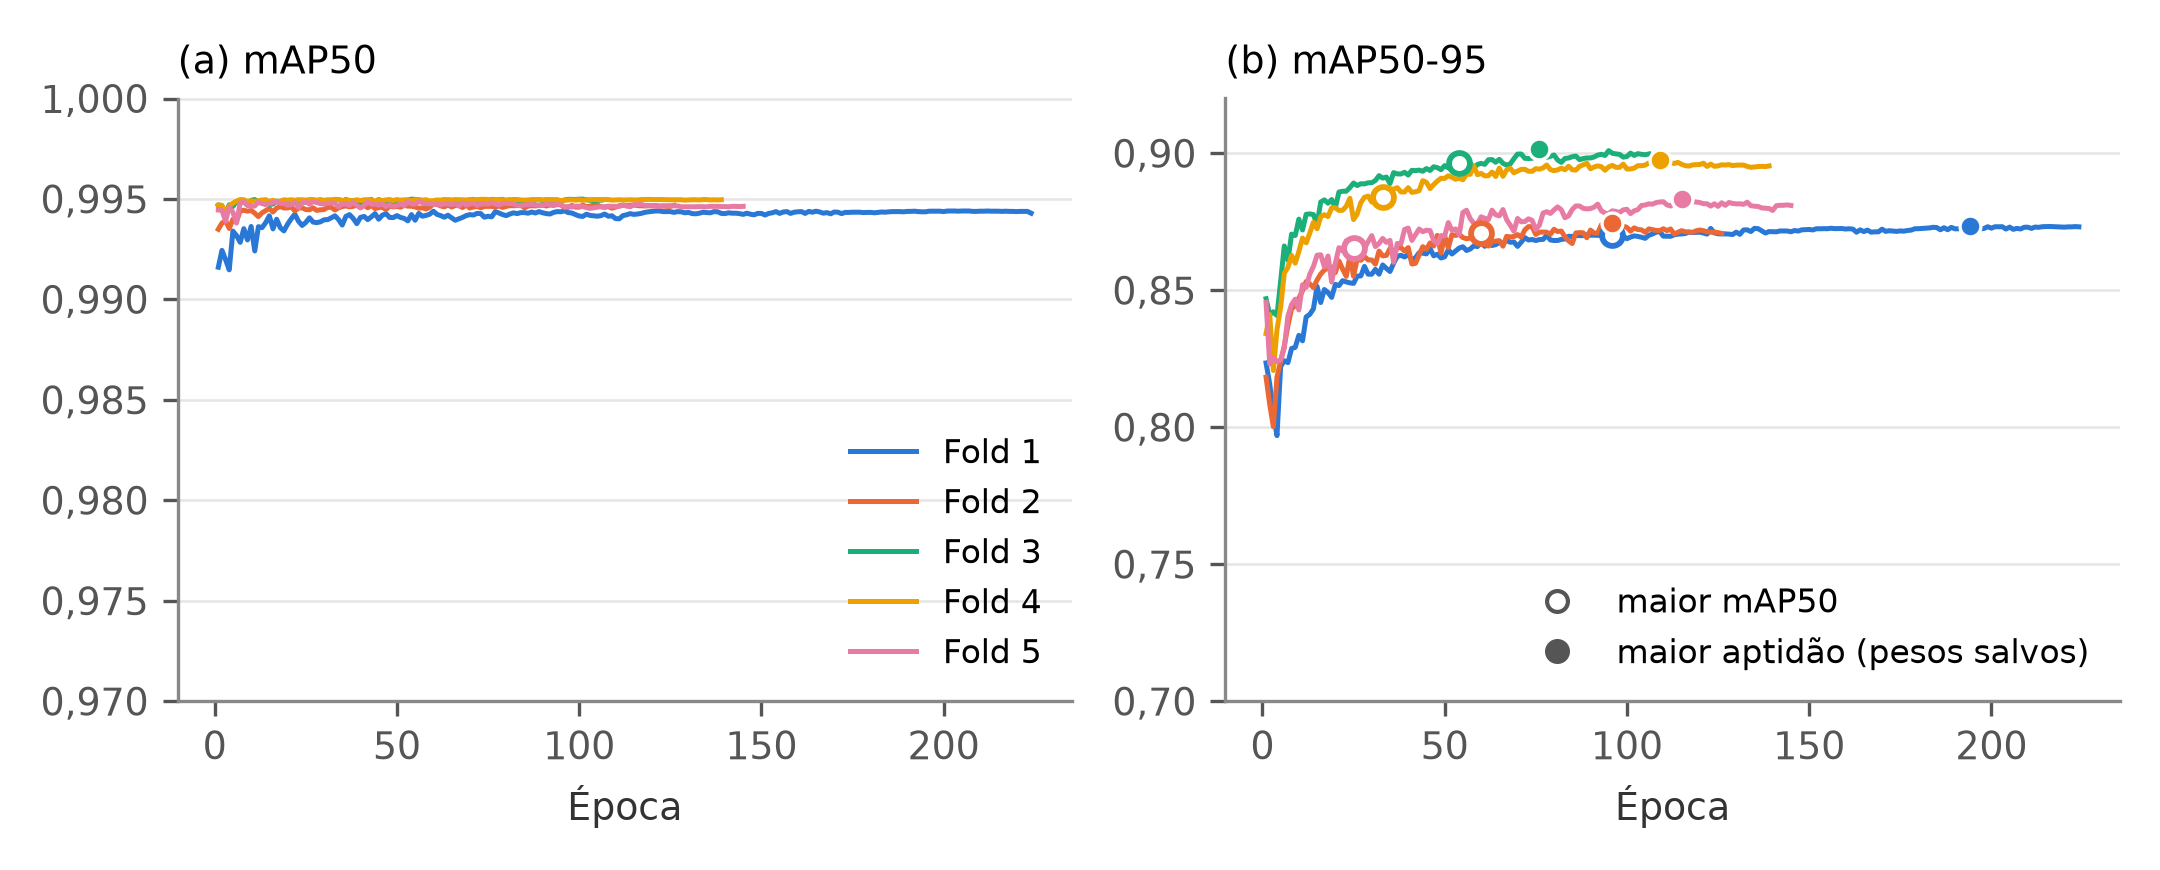
\includegraphics[width=\textwidth]{figs/baseline_curvas.png}
\caption{Evolução do mAP50 (a) e do mAP50-95 (b) de validação do baseline monolítico nos cinco \textit{folds}. Em (b), os círculos vazados indicam a época de maior mAP50 e os círculos cheios, a época de maior aptidão (pesos salvos).}
\label{fig:curvas-baseline}

Fonte: Elaborada pelo autor.
\end{figure}

A Tabela~\ref{tab:res-baseline-aptidao} mostra as métricas na época de maior aptidão, junto com a época em que cada treinamento parou e sua duração. A parada ocorreu sempre 30 épocas depois da época de maior aptidão, o que confirma que a paciência foi contada sobre essa métrica. Nesse critério, o mAP50-95 médio do baseline sobe de 0,8773 para 0,8860, e o do \textit{fold} 3 chega a 0,9015. Os cinco treinamentos somaram cerca de 15 horas.

\begin{table}[htb]
\centering
\caption{Baseline monolítico na época de maior aptidão (pesos salvos), época de parada e duração do treinamento de cada \textit{fold}.}
\label{tab:res-baseline-aptidao}
\footnotesize
\begin{tabular}{lccccc}
\hline
\textbf{Fold} & \textbf{Época (aptidão)} & \textbf{mAP50} & \textbf{mAP50-95} & \textbf{Parada} & \textbf{Duração} \\
\hline
1 & 194 & 0,9944 & 0,8733 & 224 & 4 h 39 min \\
2 & 96 & 0,9946 & 0,8745 & 126 & 2 h 29 min \\
3 & 76 & 0,9950 & 0,9015 & 106 & 2 h 05 min \\
4 & 109 & 0,9949 & 0,8974 & 139 & 2 h 45 min \\
5 & 115 & 0,9947 & 0,8832 & 145 & 3 h 05 min \\
\hline
\textbf{Média} & -- & \textbf{0,9947} & \textbf{0,8860} & -- & \textbf{15 h 03 min} (total) \\
\hline
\end{tabular}

\vspace{0.2cm}
\normalsize
Fonte: Elaborada pelo autor.
\end{table}

\section{Comparação entre Especialistas e Baseline nas Métricas Agregadas}
\label{sec:res-comparacao-metricas}

Nas métricas de validação cruzada, as duas abordagens têm desempenho muito parecido. Ambas saturam o mAP50 e têm precisão, revocação e F1-\textit{score} acima de 0,99. No mAP50-95, os especialistas variam de 0,8338 a 0,9015, e o baseline tem média de 0,8773 e melhor \textit{fold} com 0,8965.

Essa comparação, porém, não é direta, por três motivos. Primeiro, os números dos especialistas são os do melhor \textit{fold} de cada um, enquanto o valor de referência do baseline é a média dos cinco \textit{folds}; comparar o melhor caso de uma abordagem com a média da outra favorece a primeira. Comparando melhor \textit{fold} com melhor \textit{fold}, o baseline (0,8965) supera três dos quatro especialistas no mAP50-95 e fica abaixo apenas de Frontal Dia (0,9015). Segundo, cada especialista é avaliado apenas sobre o seu cenário, enquanto o baseline é avaliado sobre a união dos quatro; o mAP50-95 do baseline é uma média que mistura cenários mais fáceis e mais difíceis. Terceiro, como discutido nas seções anteriores, as tabelas usam a época de maior mAP50, que não corresponde aos pesos salvos.

A forma mais justa de comparar as duas abordagens é avaliar o baseline separadamente sobre a validação de cada cenário, no mesmo \textit{fold} e com os pesos salvos, e comparar cenário a cenário com o especialista correspondente. Essa comparação é possível porque o conjunto de validação do baseline em cada \textit{fold} é exatamente a união dos conjuntos de validação dos quatro especialistas no mesmo \textit{fold}: o particionamento foi gerado pelo mesmo procedimento, sessão a sessão, e as 8.604 imagens caem no mesmo bloco nos dois casos. Os pesos salvos (\texttt{best.pt}) de cada \textit{fold} do baseline foram então avaliados pela rotina de validação do Ultralytics, com os parâmetros padrão, sobre o subconjunto de validação de cada cenário. Como verificação, a mesma avaliação sobre a validação completa reproduziu, até a quarta casa decimal, o mAP50-95 registrado pelo treinamento na época de maior aptidão (Tabela~\ref{tab:res-baseline-aptidao}). Do lado dos especialistas, foram usadas as métricas da época de maior aptidão de cada \textit{fold}, que correspondem aos pesos salvos. A Tabela~\ref{tab:res-comparacao-cenario} resume o resultado.

\begin{table}[htb]
\centering
\caption{mAP50-95 de validação por cenário: especialista e baseline monolítico avaliados sobre o mesmo subconjunto de validação, no mesmo \textit{fold}, com os pesos salvos (média $\pm$ desvio padrão dos cinco \textit{folds}).}
\label{tab:res-comparacao-cenario}
\footnotesize
\begin{tabular}{lcccc}
\hline
\textbf{Cenário} & \textbf{Especialista} & \textbf{Baseline} & \shortstack{\textbf{Diferença}\\\textbf{(esp. $-$ base)}} & \shortstack{\textbf{\textit{Folds} com}\\\textbf{especialista melhor}} \\
\hline
Frontal Dia & 0,9017 $\pm$ 0,0042 & 0,9061 $\pm$ 0,0078 & $-$0,0044 & 1 de 5 \\
Frontal Noite & 0,8835 $\pm$ 0,0061 & 0,8859 $\pm$ 0,0078 & $-$0,0025 & 1 de 5 \\
Superior Dia & 0,8421 $\pm$ 0,0268 & 0,8477 $\pm$ 0,0291 & $-$0,0055 & 0 de 5 \\
Superior Noite & 0,8968 $\pm$ 0,0390 & 0,9101 $\pm$ 0,0284 & $-$0,0133 & 1 de 5 \\
\hline
\end{tabular}

\vspace{0.2cm}
\normalsize
Fonte: Elaborada pelo autor.
\end{table}

No mAP50, as duas abordagens continuam empatadas em todos os cenários (médias entre 0,9941 e 0,9949). No mAP50-95, o baseline teve média ligeiramente maior que o especialista nos quatro cenários e foi melhor em 17 dos 20 pares de \textit{fold} e cenário. As diferenças são pequenas, entre 0,0025 e 0,0133, menores que a variação entre \textit{folds} de um mesmo modelo nos cenários superiores, mas têm sempre o mesmo sinal. A conclusão, portanto, é que a arquitetura MoE não demonstra superioridade sobre o baseline nas métricas agregadas de detecção; na comparação cenário a cenário, é o baseline que fica levemente à frente. No regime de dados deste trabalho, um único YOLOv8m consegue aprender uma representação conjunta das quatro combinações de perspectiva e iluminação tão boa quanto, ou ligeiramente melhor que, a de cada especialista, possivelmente porque é treinado com quatro vezes mais imagens.

\section{Avaliação em Vídeos de Teste}
\label{sec:res-videos}

\subsection{Verificação de Vazamento}
\label{subsec:res-vazamento}

A Tabela~\ref{tab:res-vazamento} mostra o resultado da verificação de vazamento descrita na Seção~\ref{subsec:videos-teste}. Na primeira rodada, feita com o pré-filtro por \textit{hash}, nenhum dos quatro vídeos foi identificado como recorte de uma sessão de treino: nos três vídeos em que algum par passou pelo pré-filtro, o menor MSE ficou entre 1.326,8 e 2.546,8, e no vídeo Superior Dia nenhum par passou. Essa rodada, porém, tinha duas fragilidades. O pré-filtro comparava apenas 12 quadros do vídeo com uma amostra das imagens de cada sessão e podia descartar pares próximos, e a escolha das sessões candidatas dependia da data escrita no nome do arquivo de teste, que estava errada no vídeo Superior Noite (o nome indica 29 de abril, mas a marcação gravada nos quadros indica 26 de abril). A tabela apresenta, por isso, o resultado da verificação exaustiva, que compara todos os quadros com todas as imagens da mesma câmera, e a comparação da marcação de hora dos vídeos com o intervalo coberto por cada sessão.

\begin{table}[htb]
\centering
\caption{Verificação de vazamento entre os vídeos de teste e as sessões da base de detecção (busca exaustiva por MSE contra todas as imagens da mesma câmera).}
\label{tab:res-vazamento}
\footnotesize
\begin{tabular}{lcccc}
\hline
\shortstack{\textbf{Vídeo}\\\textbf{de teste}} & \shortstack{\textbf{Câmera,}\\\textbf{data e hora}} & \shortstack{\textbf{Sessão que cobre}\\\textbf{o horário}} & \shortstack{\textbf{Menor}\\\textbf{MSE}} & \textbf{Resultado} \\
\hline
Frontal Dia & Cam03, 04/05, 14h10 & nenhuma & 1.232,3 & sem vazamento \\
Frontal Noite & Cam03, 26/04, 18h40 & Cam03, 26/04, 18h17--19h16 & 11,9 & mesma sessão \\
Superior Dia & Cam04, 29/04, 12h50 & nenhuma & 2.148,6 & sem vazamento \\
Superior Noite & Cam04, 26/04, 20h45 & nenhuma & 941,4 & sem vazamento \\
\hline
\end{tabular}

\vspace{0.2cm}
\normalsize
Fonte: Elaborada pelo autor.
\end{table}

Em três vídeos, o resultado se confirma. Os vídeos Frontal Dia e Superior Dia foram gravados em dias sem nenhuma sessão da mesma câmera na base. O vídeo Superior Noite foi gravado às 20h45 de 26 de abril, e as três sessões da Cam04 nesse dia cobrem os intervalos de 0h07 a 1h06, de 4h06 a 5h06 e de 18h06 a 19h05; o vídeo começa, portanto, 1 hora e 40 minutos depois do fim da sessão mais próxima, e o menor MSE (941,4) está na faixa de duas cenas diferentes.

O vídeo Frontal Noite, por outro lado, é um trecho de uma sessão da base. A sessão \texttt{Cam03\_2025\_04\_26\_18\_17\_10} não é um trecho contínuo de poucos segundos: seus 140 quadros cobrem uma hora de gravação, das 18h17 às 19h16, e o vídeo de teste, gravado às 18h40, está dentro desse intervalo. O quadro 54 da sessão, registrado às 18h40min17s, 4 segundos depois do último quadro do vídeo, tem MSE de 11,9 em relação a ele, abaixo do limiar de duplicata. A primeira rodada não detectou esse caso porque o pré-filtro não levou esse par à comparação por MSE. Nos \textit{folds} 1, 4 e 5, esse quadro está no treino; no \textit{fold} 3, cujos pesos foram usados tanto pelo especialista Frontal Noite quanto pelo baseline nos testes em vídeo, ele está na validação, e a imagem de treino mais próxima do vídeo é o quadro 40 da mesma sessão, cerca de seis minutos antes, com MSE de 85,2. Não há, portanto, quadro idêntico ao do vídeo no treino dos modelos testados, mas o vídeo vem da mesma gravação, com a mesma câmera, a mesma iluminação e os animais em posições parecidas. O vídeo Frontal Noite não é, assim, um teste independente, e o resultado da contagem nesse cenário deve ser lido como o de um trecho de uma sessão vista no treino. Como as duas abordagens usaram o mesmo \textit{fold} e, portanto, as mesmas imagens dessa sessão no treino, a comparação entre elas nesse vídeo continua sendo feita em condições iguais.

\subsection{Roteamento}
\label{subsec:res-roteamento-videos}

A rede de roteamento escolheu o cenário correto nos quatro vídeos. A confiança da escolha, isto é, a probabilidade atribuída pela \textit{softmax} ao cenário escolhido, foi de 99,32\% em Frontal Dia, 99,38\% em Superior Dia e 99,99\% em Superior Noite. Em Frontal Noite, foi de apenas 62,67\%.

Mesmo correta, uma confiança de 62,67\% indica que, para o primeiro quadro desse vídeo, a rede distribuiu uma parte considerável da probabilidade entre outros cenários. Isso mostra que o acerto total na validação (Seção~\ref{subsec:res-treino-roteamento}) superestima a margem de segurança da rede em vídeos novos, e que o roteamento feito com base em um único quadro tem, nesse cenário, pouca folga. Um fator que pode contribuir é que Frontal Noite é a classe com menos imagens na base da rede de roteamento (80, contra 560 de Frontal Dia).

Para investigar esse caso, a rede de roteamento foi aplicada novamente ao primeiro quadro e a todos os 80 quadros de cada vídeo de teste. No primeiro quadro do vídeo Frontal Noite, a probabilidade restante foi para Superior Noite (31,4\%), Frontal Dia (5,2\%) e Superior Dia (0,6\%). A confiança baixa não é uma particularidade desse quadro: a rede escolheu Frontal Noite em todos os 80 quadros do vídeo, mas sempre com confiança entre 58,5\% e 62,7\%, e sempre com cerca de 30\% para Superior Noite. Nos outros três vídeos, a confiança ficou acima de 98,6\% em todos os quadros. O quadro também não tem nada de incomum: a exposição é normal, e os animais estão no centro da baia, longe da câmera.

A explicação mais provável está na base da rede de roteamento (Seção~\ref{subsec:base-roteamento}). A classe Frontal Noite foi treinada com um único vídeo de 10 segundos da câmera Cam01, enquanto o vídeo de teste vem da câmera Cam03, que nenhuma imagem da base de roteamento representa. As duas câmeras frontais estão em posições diferentes e têm enquadramentos diferentes da baia. À noite, sem a informação de cor, a distinção entre as perspectivas depende só da geometria da cena, e um enquadramento que a rede não viu no treino pode ficar, para ela, a meio caminho entre as duas classes noturnas. De dia, a mesma câmera Cam03 foi classificada com mais de 98\% de confiança, possivelmente porque a classe Frontal Dia tem sete vídeos e porque a cor ajuda a separar os cenários. Como a confiança é baixa de forma sistemática em todos os quadros, classificar vários quadros e decidir pela média das probabilidades não aumentaria a margem nesse vídeo, embora proteja contra um primeiro quadro atípico. A forma de tornar o roteamento mais seguro é incluir na base de roteamento imagens de todas as câmeras usadas, em especial da Cam03 e da Cam04.

\subsection{Contagem de Animais}
\label{subsec:res-contagem}

A Tabela~\ref{tab:res-contagem} apresenta o total de caixas detectadas por cada abordagem em cada vídeo. Como os oito animais estão na baia em todos os quadros, o valor esperado é de 640 caixas por vídeo.

\begin{table}[htb]
\centering
\caption{Total de caixas detectadas nos vídeos de teste (80 quadros cada; valor esperado de $8 \times 80 = 640$).}
\label{tab:res-contagem}
\begin{tabular}{lccc}
\hline
\textbf{Cenário} & \textbf{Baseline} & \textbf{MoE} & \textbf{Esperado} \\
\hline
Frontal Dia & 623 & 640 & 640 \\
Frontal Noite & 643 & 640 & 640 \\
Superior Dia & 532 & 640 & 640 \\
Superior Noite & 663 & 640 & 640 \\
\hline
\end{tabular}

\vspace{0.2cm}
Fonte: Elaborada pelo autor.
\end{table}

A arquitetura MoE produziu exatamente 640 caixas nos quatro vídeos, com oito caixas em cada um dos 320 quadros. O baseline errou a contagem nos quatro vídeos, ora para menos, ora para mais. A análise quadro a quadro mostra dois padrões de erro diferentes.

O primeiro é a subdetecção. No vídeo Superior Dia, o baseline não chegou a oito caixas em nenhum dos 80 quadros, oscilando entre cinco e sete, e o total ficou 108 caixas abaixo do esperado. Nesse vídeo, os animais aparecem agrupados e encostados uns nos outros, e o baseline tende a deixar de fora animais parcialmente encobertos pelos vizinhos. No vídeo Frontal Dia, o total ficou 17 caixas abaixo do esperado.

O segundo é a sobredetecção. No vídeo Superior Noite, 26 dos 80 quadros tiveram mais de oito caixas, chegando a dez, e no vídeo Frontal Noite isso ocorreu em 4 dos 80 quadros. Nesses quadros, as caixas excedentes não são falsos positivos sobre o fundo: são caixas duplicadas sobre um animal que já tinha sido detectado. O IoU entre a caixa duplicada e a original chegou a 0,64, abaixo do limiar de 0,7 da supressão de não máximos, de modo que as duas caixas foram mantidas pelo pós-processamento. Nos totais da Tabela~\ref{tab:res-contagem}, a sobredetecção pode encobrir parte da subdetecção; o total de Frontal Noite (643), por exemplo, está próximo do esperado, mas inclui quadros com caixas a mais.

A Figura~\ref{fig:comparacao-videos} mostra exemplos desses erros, com o baseline à esquerda e o especialista correspondente à direita, no mesmo quadro de cada vídeo. Em Frontal Dia (a, b) e Superior Dia (e, f), o baseline detecta seis e cinco animais, respectivamente, e o especialista detecta os oito. Em Frontal Noite (c, d) e Superior Noite (g, h), o baseline atribui duas caixas a um mesmo animal, ambas com confiança de pelo menos 0,73, enquanto o especialista delimita cada animal com uma única caixa.

\begin{figure}[p]
\centering
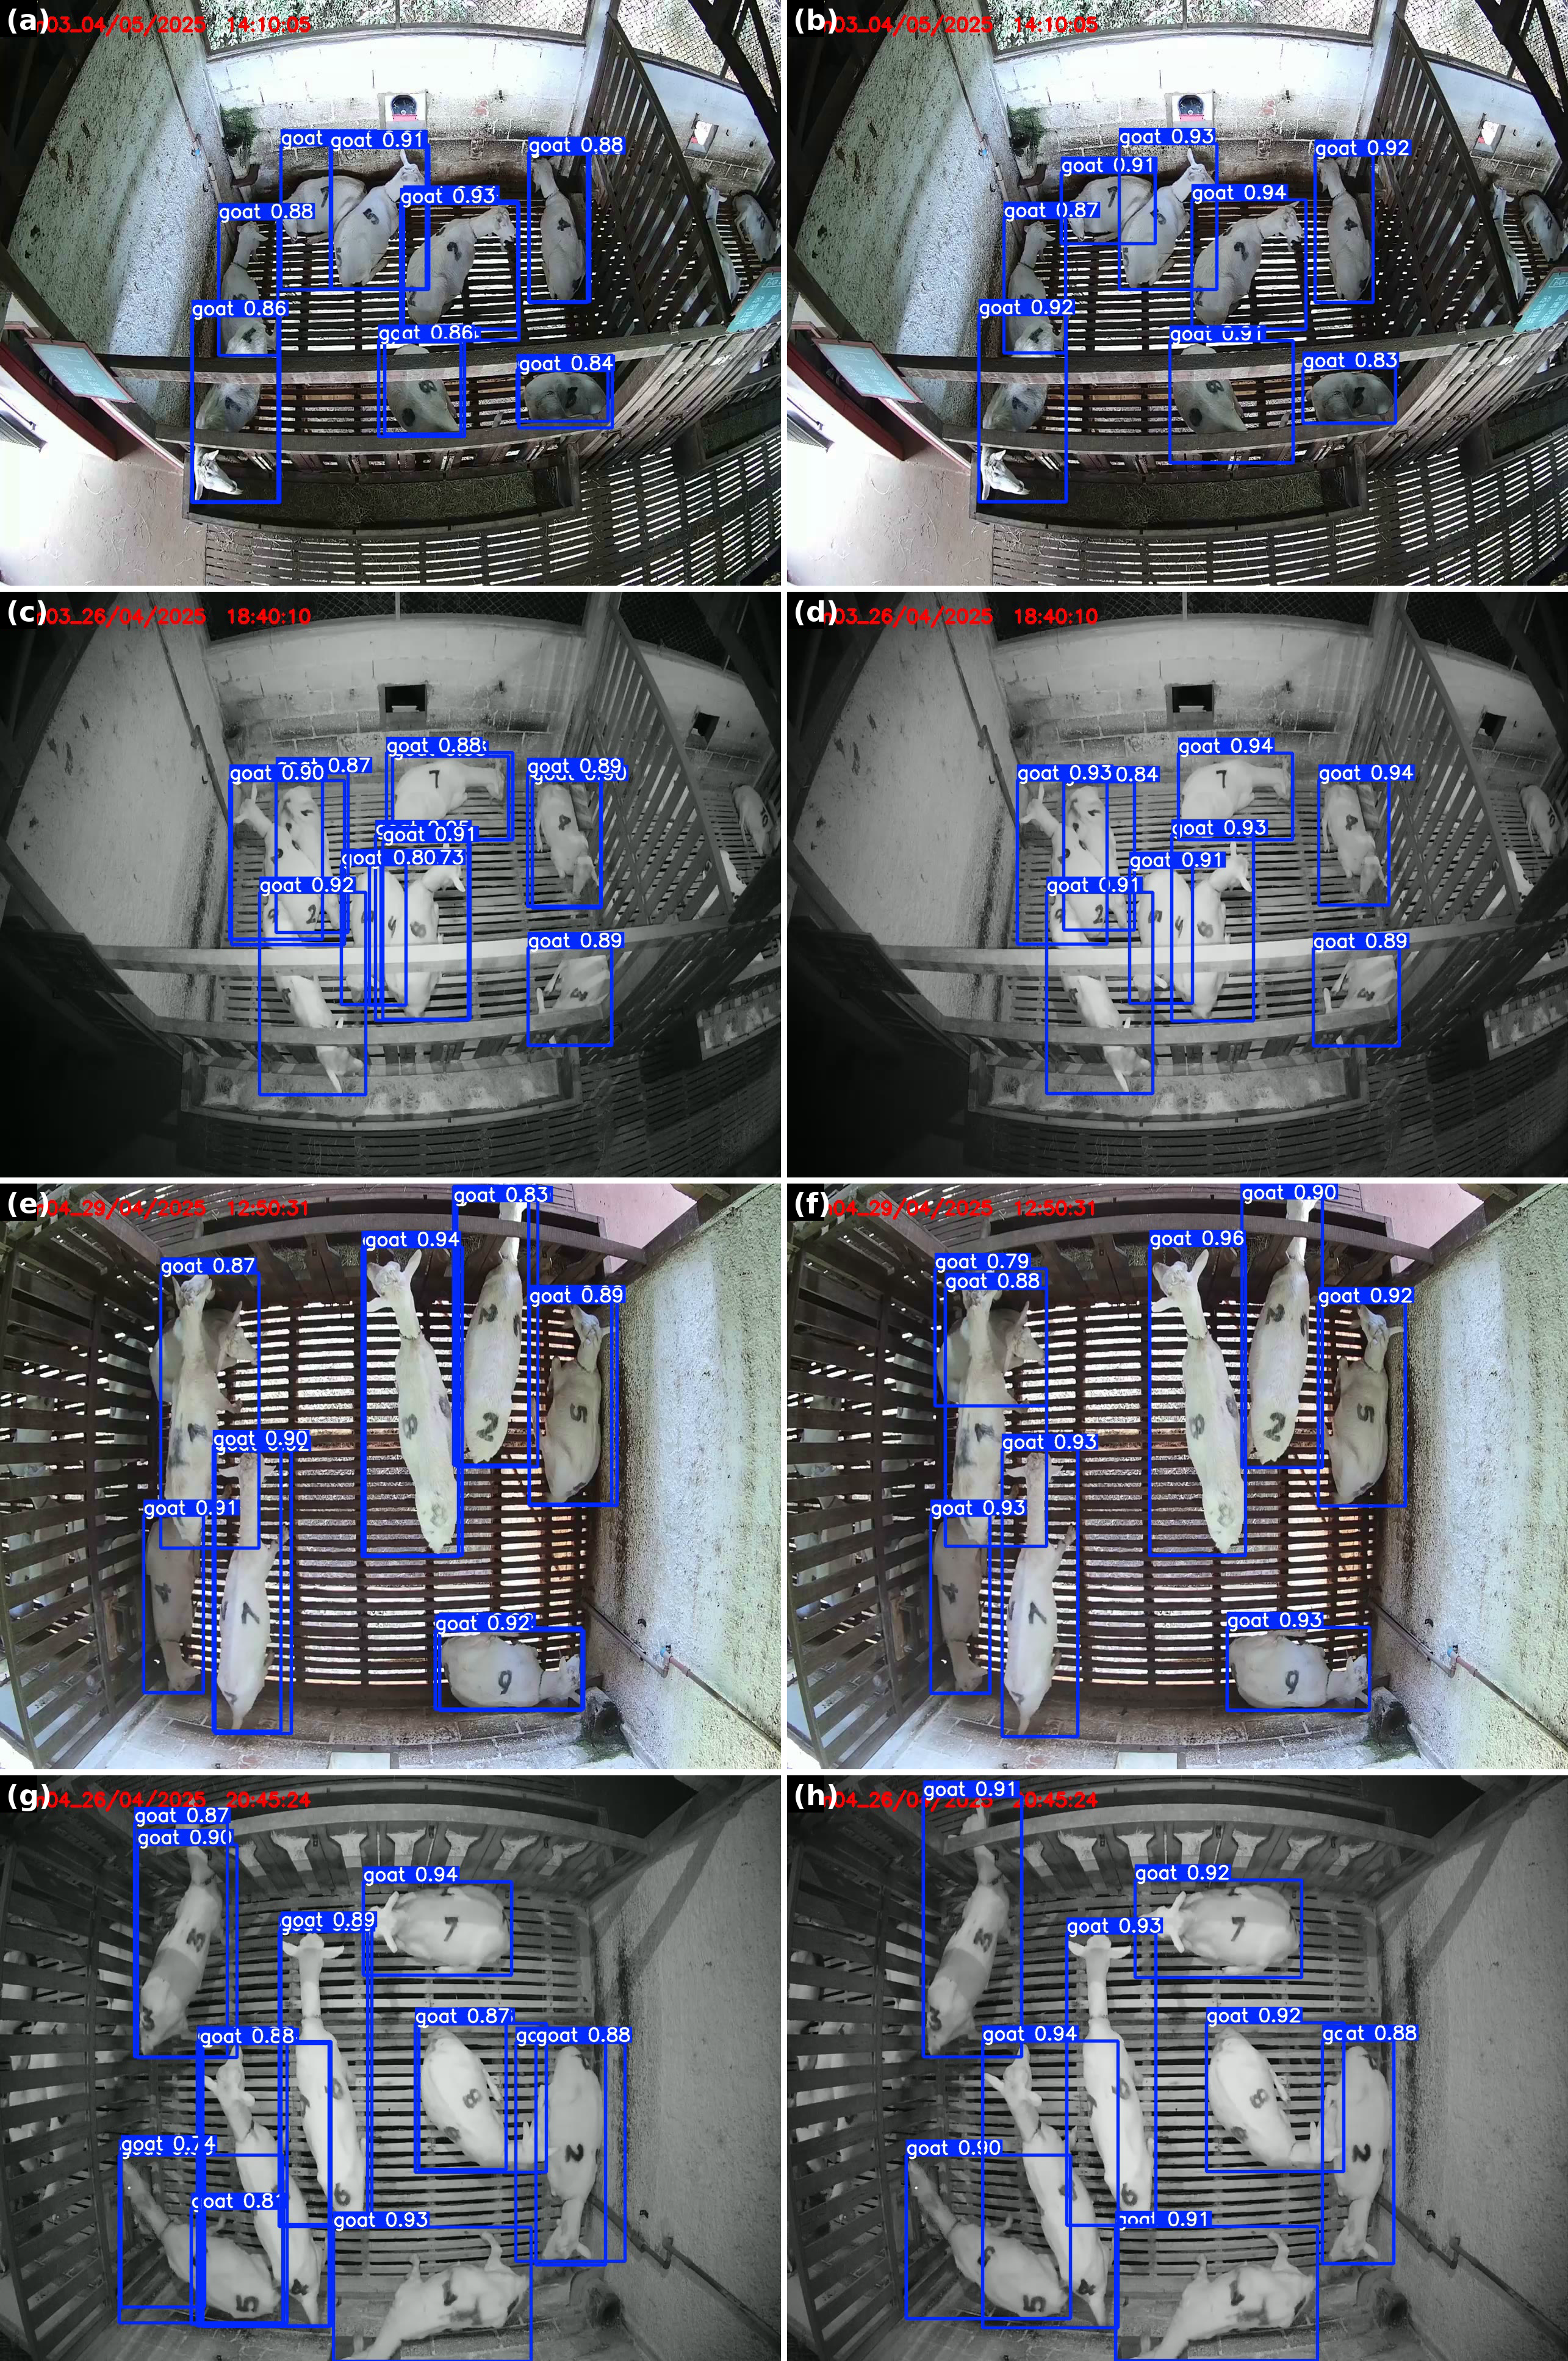
\includegraphics[width=0.82\textwidth]{figs/comparacao_overall_moe.png}
\caption{Baseline monolítico (esquerda) e especialista MoE correspondente (direita), no mesmo quadro do mesmo vídeo de teste: (a)-(b) Frontal Dia, quadro 10 (6 e 8 caixas); (c)-(d) Frontal Noite, quadro 55 (9 e 8 caixas); (e)-(f) Superior Dia, quadro 62 (5 e 8 caixas); (g)-(h) Superior Noite, quadro 6 (10 e 8 caixas).}
\label{fig:comparacao-videos}

Fonte: Elaborada pelo autor.
\end{figure}

As 2.560 caixas produzidas pelos especialistas nos quatro vídeos tiveram confiança entre 0,74 e 0,96, com média de 0,91. Como o limiar de confiança usado foi 0,7, nenhuma caixa ficou muito perto do limite de corte, o que indica que a contagem correta não dependeu de um ajuste fino desse limiar.

\section{Discussão}
\label{sec:res-discussao}

\subsection{Por que as Métricas Agregadas não Mostram a Diferença}
\label{subsec:disc-metricas}

Os resultados das Seções~\ref{sec:res-comparacao-metricas} e~\ref{sec:res-videos} parecem contraditórios. Nas métricas de validação cruzada, as duas abordagens empatam; na contagem em vídeo, o baseline erra nos quatro cenários e o MoE acerta todos os quadros. Há duas razões principais para essa diferença.

A primeira é que as duas avaliações medem coisas diferentes. O mAP resume a qualidade do detector em todos os limiares de confiança, ordenando as caixas da mais confiante para a menos confiante. Uma caixa duplicada sobre um animal já detectado conta como um falso positivo, mas, se tiver confiança menor que a das caixas corretas, entra no fim dessa ordenação e reduz pouco a área sob a curva de precisão e revocação. Na contagem, em um limiar fixo de 0,7, a mesma caixa duplicada soma um animal a mais no quadro. Do mesmo modo, um animal detectado com confiança 0,6 contribui para o mAP, mas desaparece da contagem com o limiar de 0,7.

A segunda é que os vídeos de teste são mais distantes do treino que os blocos de validação. Como discutido na Seção~\ref{subsec:limitacoes-protocolo}, a validação usa trechos de sessões cujos outros trechos foram vistos no treino. Os vídeos de teste vêm de momentos diferentes, com outras posições e agrupamentos dos animais, com a exceção do vídeo Frontal Noite, que é um trecho de uma sessão da base (Seção~\ref{subsec:res-vazamento}). É razoável supor que, diante de dados realmente novos, as diferenças entre as abordagens apareçam mais do que na validação cruzada, e foi o que se observou.

\subsection{Interpretação do Desempenho dos Especialistas}
\label{subsec:disc-especialistas}

Os especialistas mantiveram a contagem correta nos quatro cenários, inclusive naqueles em que o baseline mais errou. Uma interpretação compatível com esses resultados é que cada especialista, treinado com imagens de uma única combinação de perspectiva e iluminação, ajusta o tamanho e a forma das caixas e o nível de confiança a uma distribuição visual mais homogênea. O baseline precisa conciliar, nos mesmos parâmetros, animais grandes e vistos de lado nas câmeras frontais com animais menores e vistos de cima nas câmeras superiores, em imagens coloridas e em infravermelho. Os erros do baseline foram diferentes em cada cenário (subdetecção nos cenários diurnos, sobredetecção nos noturnos), o que é coerente com um modelo cujo ajuste é um compromisso entre cenários. Essa interpretação, no entanto, não foi testada diretamente, e outros fatores, como diferenças entre os \textit{folds} escolhidos, podem contribuir para o resultado.

\subsection{Vantagens e Custos da Arquitetura Modular}
\label{subsec:disc-modularidade}

Além da estabilidade da contagem, a arquitetura MoE tem propriedades estruturais que as métricas não medem. Um novo cenário, como uma nova câmera ou uma nova baia, pode ser incorporado treinando um novo especialista e acrescentando uma classe à rede de roteamento, sem retreinar os especialistas existentes. Uma dificuldade própria de um cenário, como o mAP50-95 mais baixo da perspectiva superior, fica restrita ao especialista daquele cenário e pode ser tratada nele, por exemplo com mais dados, sem risco de piorar os demais. E a rede de roteamento informa, para cada vídeo, qual especialista foi usado e com que confiança, um sinal que pode ser registrado e auditado e que não existe em um detector único.

Esses benefícios têm custos. O sistema tem cinco modelos em vez de um, e o treinamento dos especialistas e da rede de roteamento exige mais etapas que o de um detector único. O roteamento é um ponto único de falha: um erro no primeiro quadro leva o vídeo inteiro a um especialista inadequado, e o caso de Frontal Noite mostrou que a margem da rede de roteamento pode ser pequena em vídeos novos. No custo de inferência, as duas abordagens se equivalem, pois executam um único YOLOv8m por quadro, e a rede de roteamento é executada apenas uma vez por vídeo. Nos testes, tanto o \textit{pipeline} MoE quanto o baseline processaram cada vídeo de 80 quadros em menos de 3 segundos na GPU usada nos experimentos; esses tempos podem incluir o aquecimento inicial do modelo e não foram medidos de forma controlada, e não foram feitas medições em equipamentos de menor capacidade.

\subsection{Limitações}
\label{subsec:disc-limitacoes}

Os resultados deste capítulo devem ser lidos com as seguintes limitações. A validação cruzada não separa sessões inteiras entre treino e validação, e a validação da rede de roteamento foi feita com divisão aleatória por quadro. As métricas das Tabelas~\ref{tab:res-especialistas} e~\ref{tab:res-baseline} correspondem à época de maior mAP50, e não aos pesos salvos, embora a comparação cenário a cenário (Tabela~\ref{tab:res-comparacao-cenario}) use os pesos salvos. A avaliação em vídeo usou um único vídeo por cenário, com 80 quadros cada, sem rótulos, e o vídeo Frontal Noite pertence a uma sessão da base de detecção. A base da rede de roteamento não contém imagens das câmeras Cam03 e Cam04, de onde vêm os vídeos de teste. Além disso, a métrica de contagem não distingue um animal perdido de um compensado por uma caixa duplicada no mesmo quadro. Por fim, toda a base vem de uma única baia, com o mesmo rebanho de oito animais, e o comportamento dos modelos em outras instalações não foi avaliado. Essas limitações não invalidam o padrão observado, que foi consistente nos quatro cenários, mas restringem o alcance das conclusões e orientam os trabalhos futuros discutidos no Capítulo~6.
